\chapter{Results}
\label{ch:results}
The final results of this analysis are the polynomial fit to the \mt~distribution in the SVJ Fit SR, and the BumpHunter evaluation of the \mt~distribution in the Discovery SR. In the SVJ Fit region, systematic uncertainties are evaluated on the signal model, and limits on the observed $Z'$ production cross section are set. 

\section{SVJ Fit Result}
\label{sec:results_svj}
Figure~\ref{fig:unblinded_PFN_bonly} shows the unblinded \mt~spectrum in the SVJ Fit SR with a background-only fit. 
The fit is successful and has a p-value of 0.265, indicating the data is compatible with the background hypothesis. 
Table~\ref{tab:unblinded_params} gives the values and uncertainties for the five parameters of the polynomial fit function given in Equation~\ref{eq:bkgpoly}. 
\begin{figure}[!htbp]
\centering
   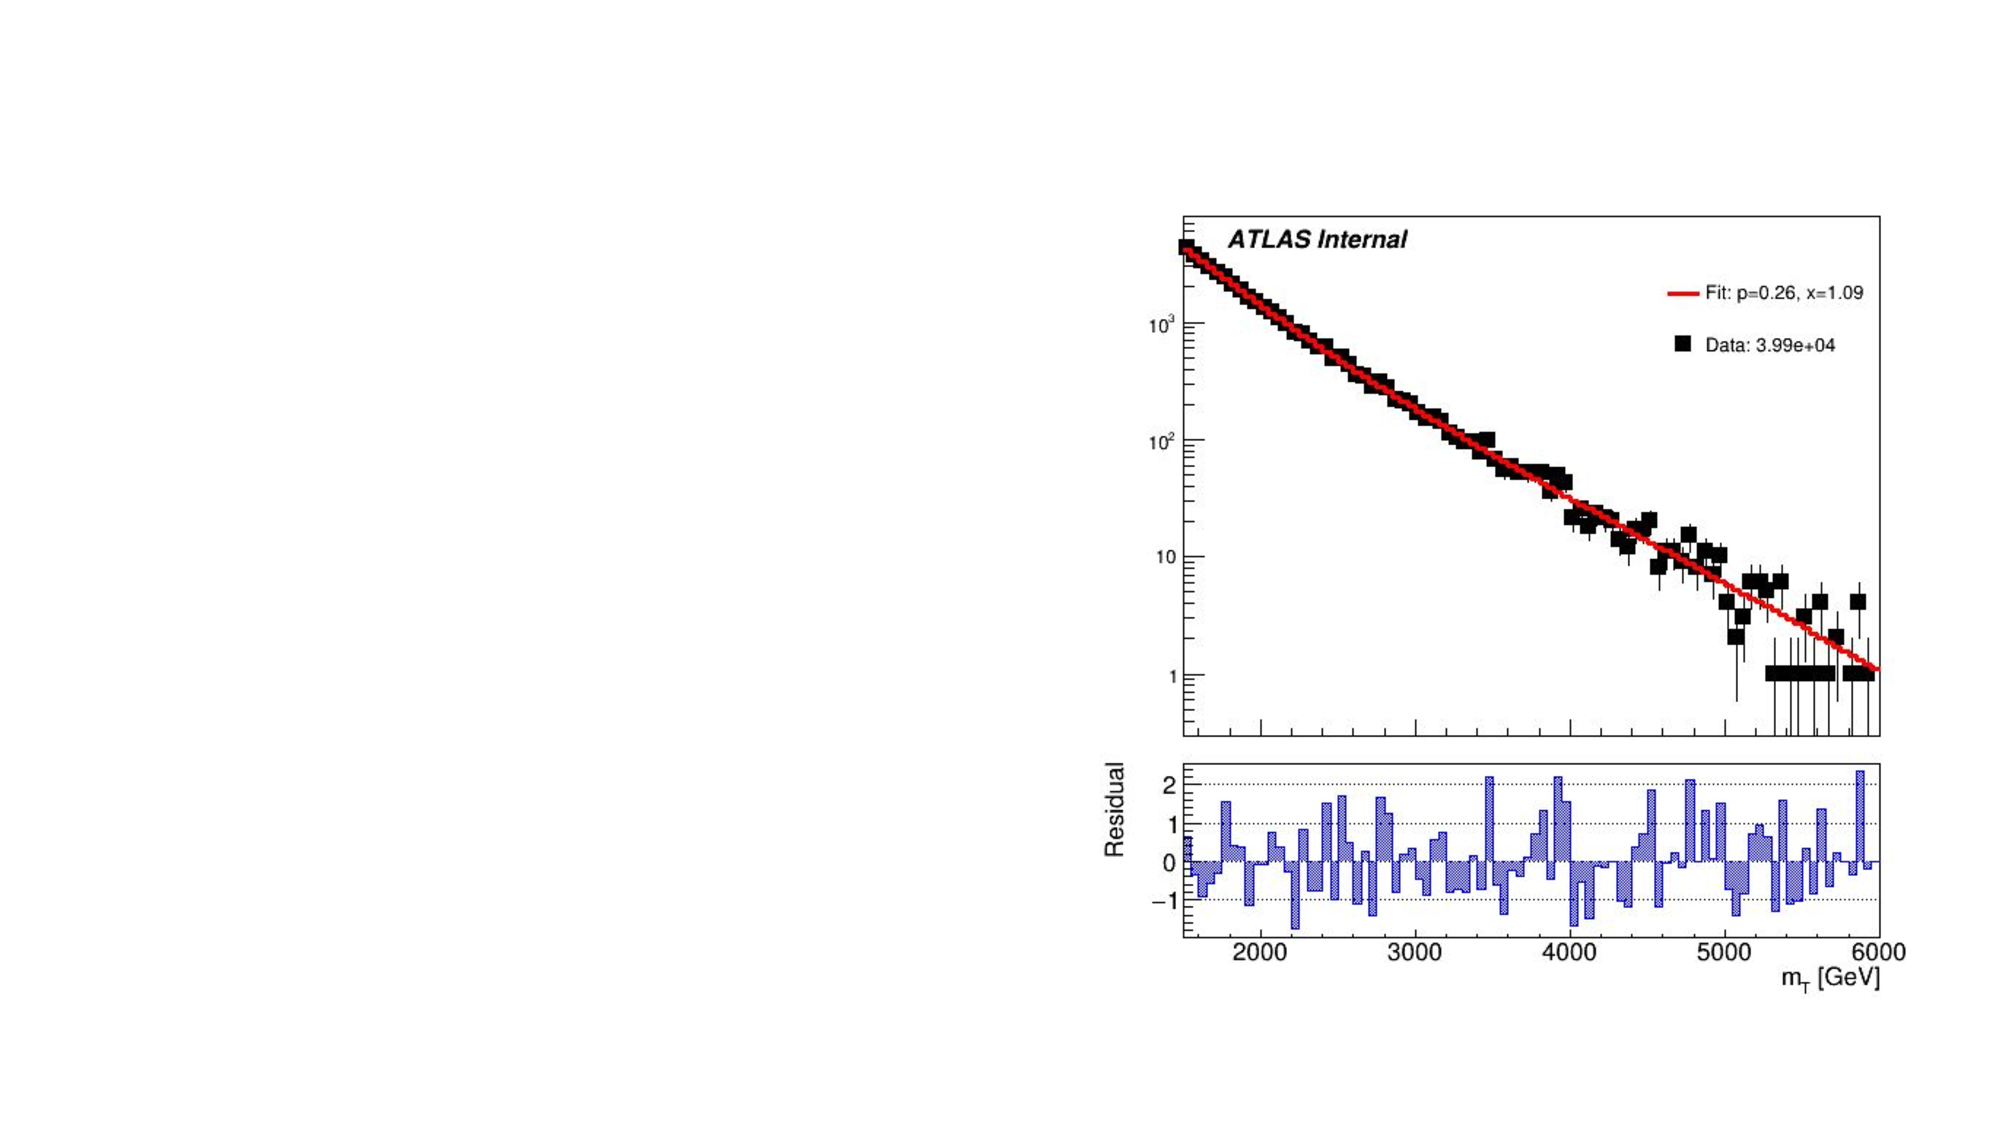
\includegraphics[width=0.5\textwidth]{figures/results/unblinded_PFN_bonly}
    \caption{\mt~in the unblinded SVJ Fit SR with a background-only fit (p-value = 0.265).
    \label{fig:unblinded_PFN_bonly}}
\end{figure}

\begin{table}[!htbp]
\centering
   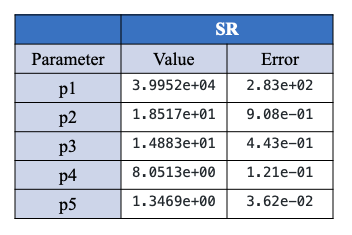
\includegraphics[width=0.45\textwidth]{figures/results/postfit_param_pfnSR}
    \caption{Post-fit parameters for the PFN SR. $p1$ can also be considered $N_{bkg}$ or the normalization factor.
    \label{tab:unblinded_params}}
\end{table}

%Figure~\ref{fig:unblinded_limits_nosyst} shows the expected and observed limits in the unblinded SR, without signal systematics considered in the fit.
%As the data was found in the b-only fit to be compatible with background, good agreement of observed and expected limits is seen.
%\begin{figure}[!htbp]
%\centering
 %  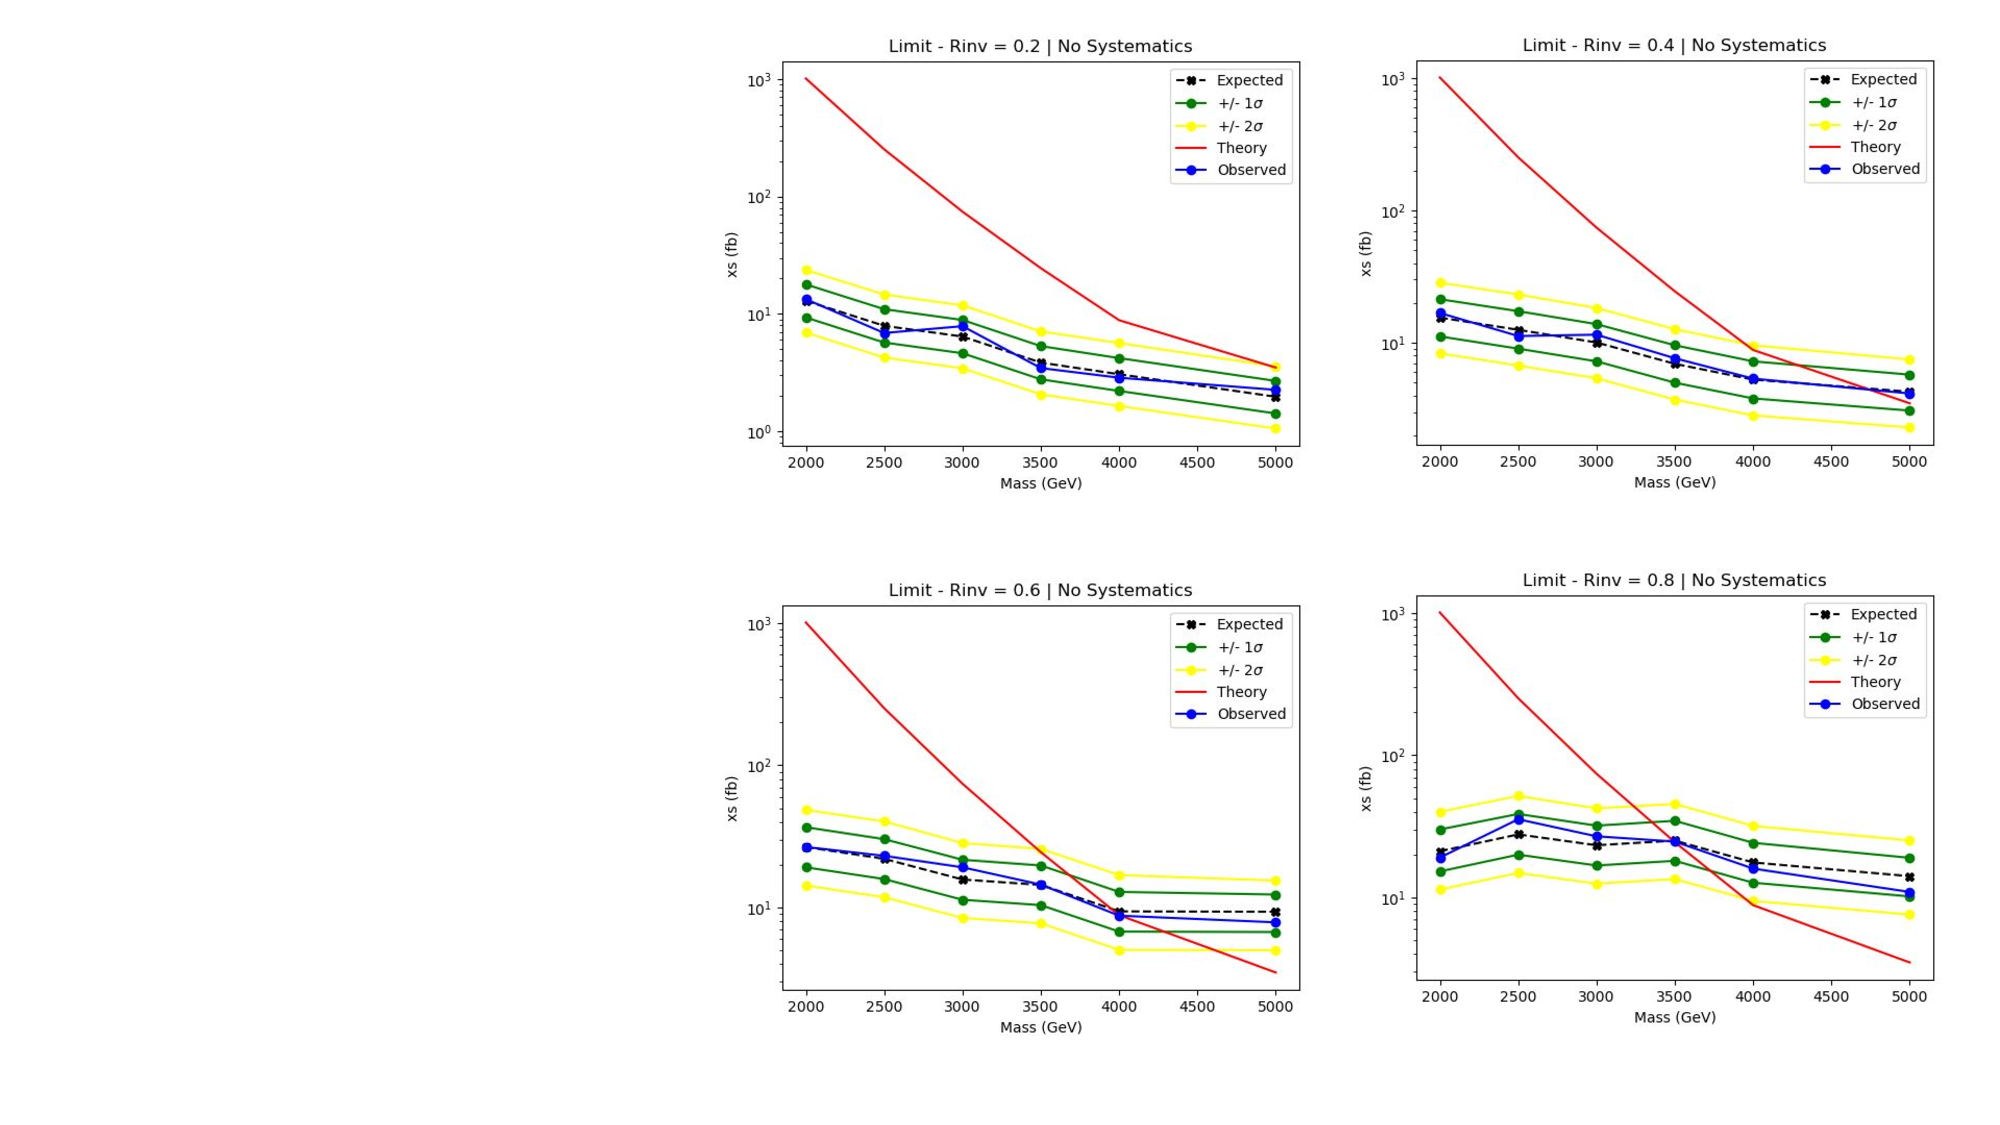
\includegraphics[width=0.95\textwidth]{figures/results/unblinded_limits_nosyst}
 %   \caption{Expected and observed 95\% CL limits in the unblinded SR, as a function of Z' masses for \rinv=0.2 (top left), 0.4 (top right), 0.6 (bottom left), 0.8 (bottom right); no systematics.
%    \label{fig:unblinded_limits_nosyst}}
%\end{figure}

\subsection{Systematics}
\label{sec:syst}
As is typically done in dijet resonance searches using a polynomial fit \cite{dijet_uncert}, the systematic uncertainties in this analysis are applied only to the signal and not to the background.
This is because the background expectation is determined entirely from the data in the SR via the polynomial fit.
Therefore the only uncertainty on the background is the statistical uncertainty, which is reflected in the uncertainty associated to each of the five freely floating parameters determined in the fit.

A variety of systematics on the signal shape and yield are considered.
The most significant of these is the \textit{spurious signal} systematic, which quantifies the level of signal observed in the absence of signal injection.
Experimental uncertainties on the luminosity and jet reconstruction are studied.
Finally, uncertainties on the MC simulation of the SVJ theory model are also considered.

%------------------------------------------------------------
\subsubsection{Spurious Signal}

The spurious signal uncertainty is assessed following the prescription in Ref.~\cite{smooth_bkg}.
Asimov pseudo-datasets as described in Section~\ref{subsec:fit_bkgonly} are used to estimate the spurious signal.
The spurious signal uncertainty is included in the fit as a systematic uncertainty on the \textit{yield} of each signal point.

The spurious signal $\text{S}_{\text{spur}}$ is quantified for each signal as the mean number of signal events fitted across 100 signal-free pseudo-data experiments. 
To determine if the amount of spurious signal is tolerable, the threshold $\text{S}_{\text{spur}}$/$\sigma_{\text{fit}} < 0.5$ is used as recommended in Ref.~\cite{smooth_bkg}.
$\sigma_{\text{fit}}$ is the standard deviation on the number of fitted signal events for each signal point across the 100 pseudo-data experiments, and represents the statistical uncertainty on the number of fitted signal events.
The approximate total uncertainty on the fitted signal event yield is therefore $\sigma_\text{tot} \approx \sqrt{\sigma_\text{fit}^2 + \text{S}_\text{spur}^2}$ with the addition of the spurious signal systematic.
The requirement $\text{S}_{\text{spur}}$/$\sigma_{\text{fit}} < 0.5$ enforces that the increase in the total measurement uncertainty $\sigma_\text{tot}$ is tolerable at < 15\% ($\sqrt{1+0.5^2} \approx 1.12$ for $\text{S}_{\text{spur}} = 0.5\sigma_\text{fit}$).

%Figure~\ref{fig:spursig_nevents} shows the determined spurious signal as a function of Z' resonance mass, for both low and high \rinv~points.
Figure~\ref{fig:spursig} shows the $\text{S}_{\text{spur}}$/$\sigma_{\text{fit}}$ metric.
The requirement for $\text{S}_{\text{spur}}$/$\sigma_{\text{fit}}$ < 0.5 is easily satisfied across the signal grid.
\begin{figure}[!htbp]
\centering
   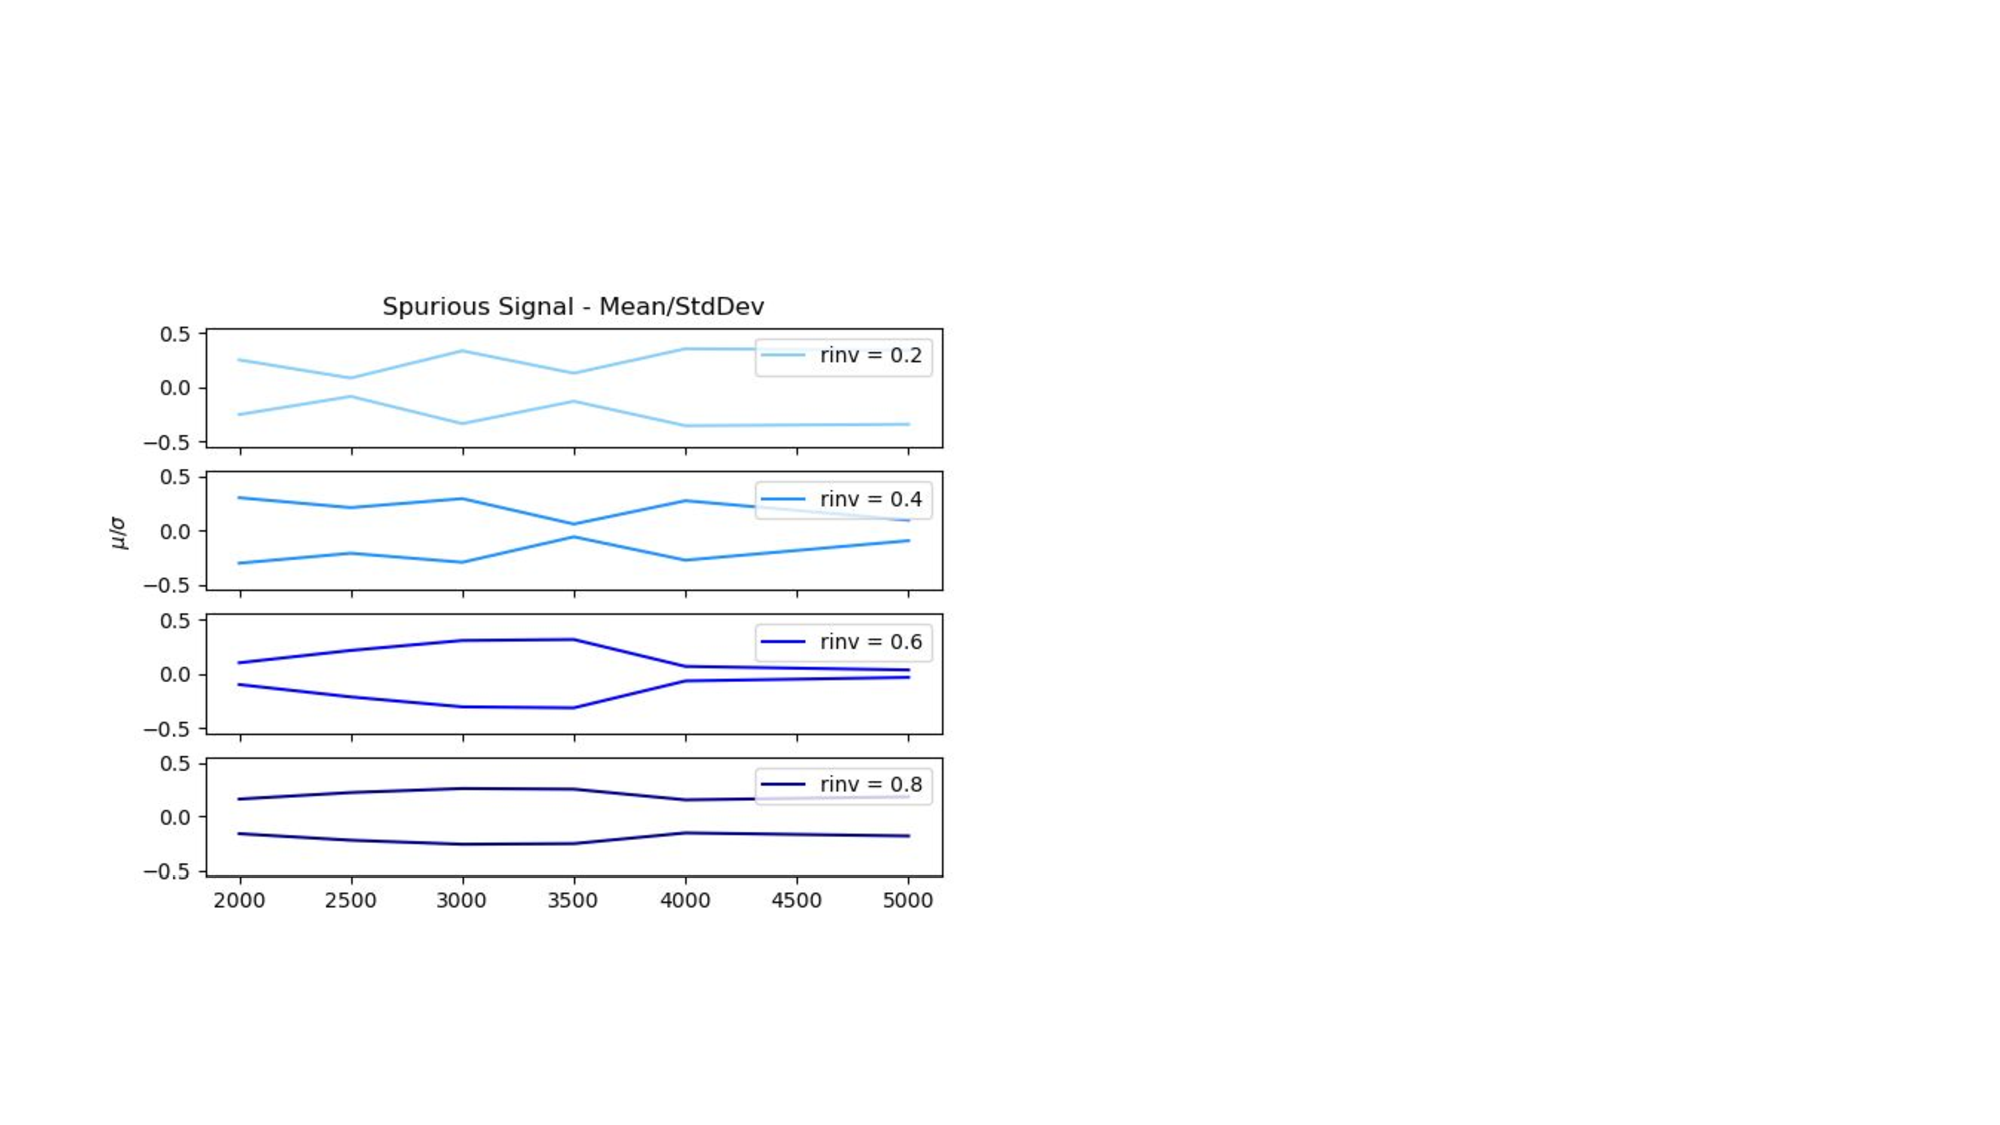
\includegraphics[width=0.6\textwidth]{figures/systs/spursig}
    \caption{Spurious signal metric as a function of resonance mass. The requirement $\text{S}_\text{spur}/\sigma_\text{fit} <0.5$ is satisfied for all signal points. 100 pseudo-data experiments are used for the measurement.
    \label{fig:spursig}}
\end{figure}

%As an additional verification of the size of the spurious signal, we perform the same check in the VR, as shown in Figure~\ref{fig:spursig_vs_mass_vr}.
%The size of the fitted spurious signal in the VR is consistent with that of the CR, indicating a good estimate of this uncertainty and extrapolation across regions.
%\begin{figure}[!htbp]
%\centering
%   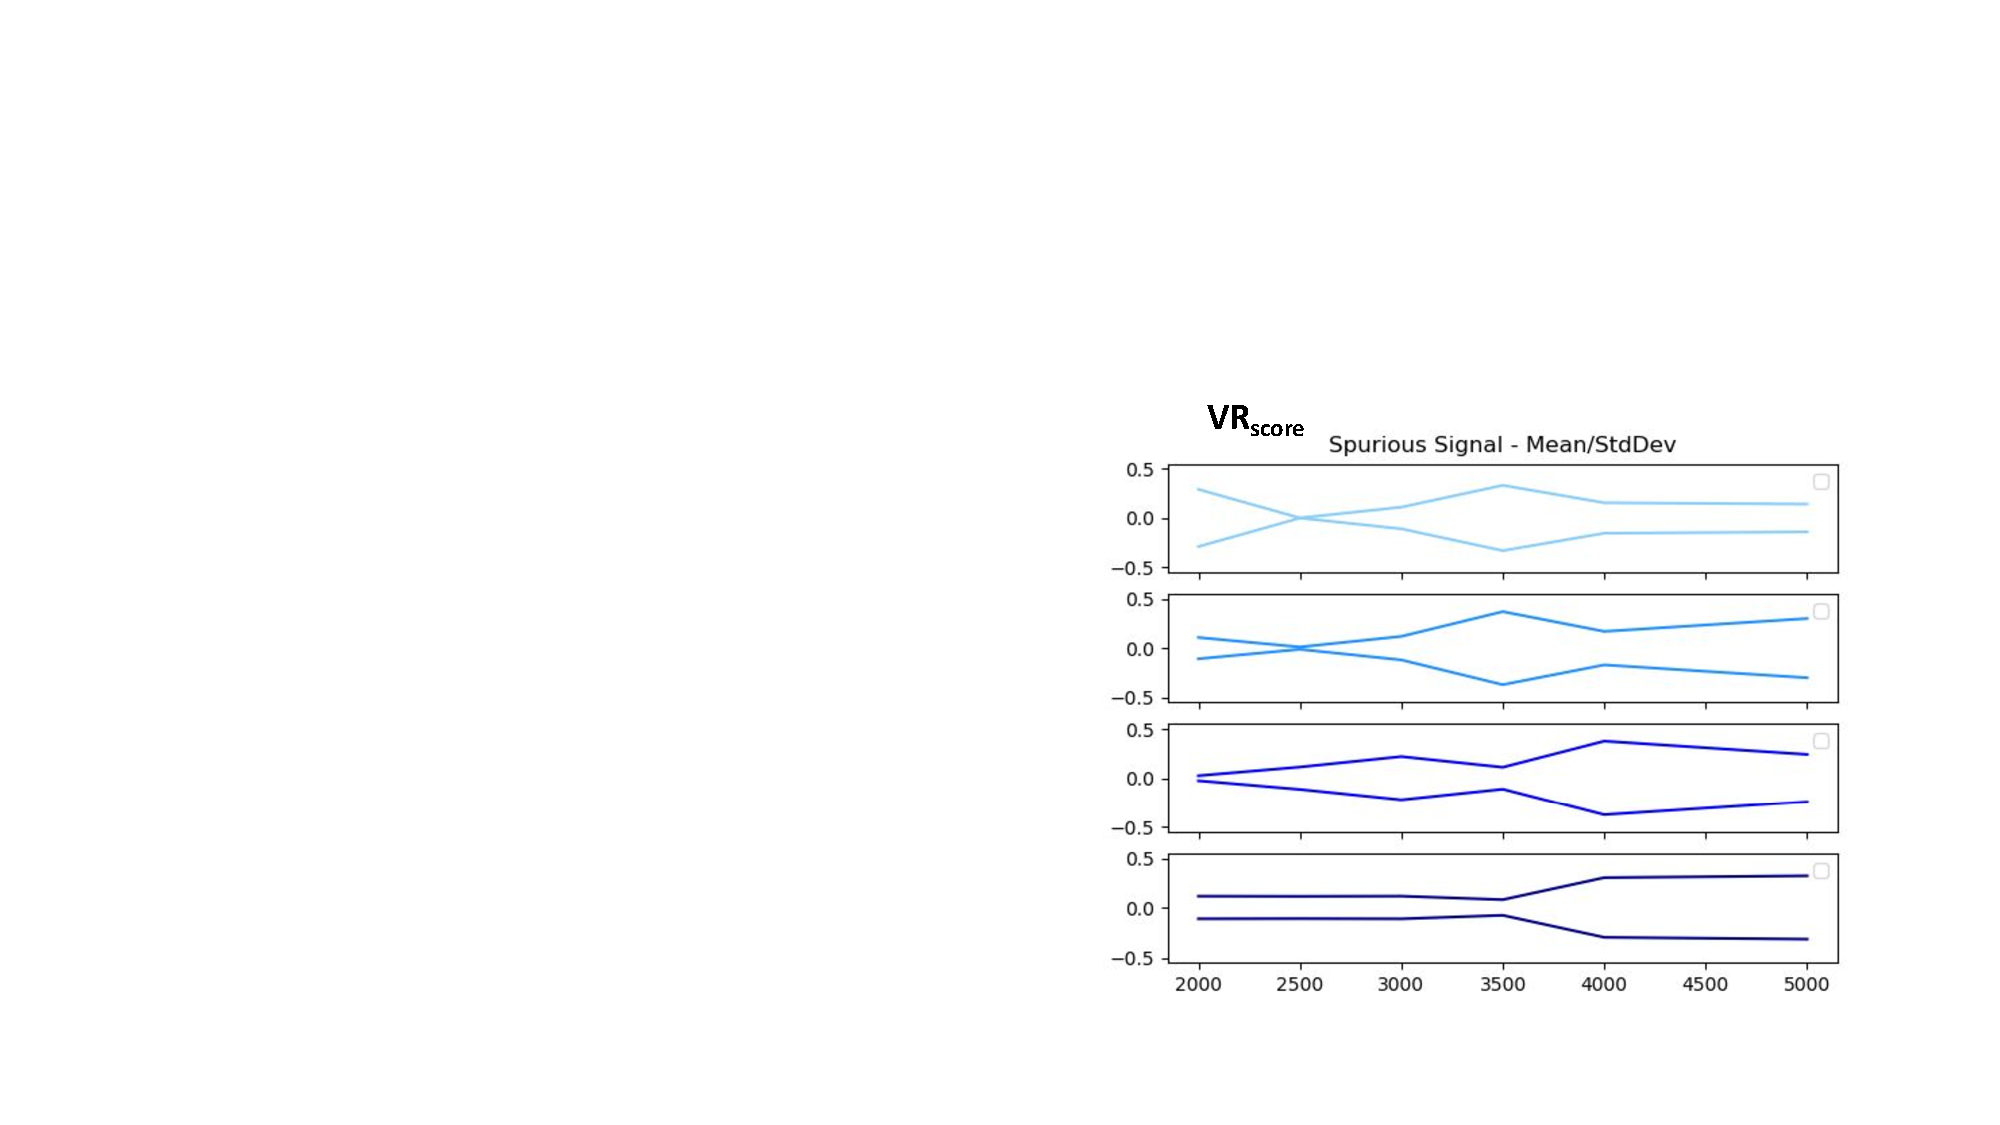
\includegraphics[width=0.6\textwidth]{figures/systs/spursig_vs_mass_vr}
%    \caption{Fitted spurious signal in the VR, consistent with the CR and within the target size of $<$ 0.5 $\sigma$.
 %   \label{fig:spursig_vs_mass_vr}}
%\end{figure}

The average size of $\text{S}_{\text{spur}}$ is 209 events, and it ranges from 23 events for some \rinv~=0.2 signals to 470 events for some \rinv~=0.8 signals.
For most points the spurious signal uncertainty is about 50\% of the expected signal yield, though it ranges from 4.2\% for $m_{Z'}$ = 2000 to over 100\% for $m_{Z'}$ = 5000 GeV.
The experimental and theory uncertainties presented in the following sections are generally negligible in the fit due to the size of the spurious signal uncertainty.
They are included for completeness, and have some impact for the $m_{Z'}$ = 2000 GeV, \rinv~= 0.2 and $m_{Z'}$ = 2500 GeV, \rinv~= 0.2 signal points, where the spurious signal uncertainty is < 5\%. 
%------------------------------------------------------------
\subsubsection{Experimental Uncertainties}
The main experimental uncertainties are on the recorded luminosity, \textit{jet energy scale}, and \textit{jet energy resolution}.
The jet energy scale (JES) corrects for the non-compensating calorimeter response and jet energy losses in passive detector material \cite{jes_jer}.
The jet energy resolution (JER) applies a correction which accounts for the spread of possible reconstructed energies for a jet with a fixed true energy, as determined in simulation.
Systematics uncertainties on the JES and JER processes must be considered for any analysis using reconstructed jets.

A flat yield uncertainty of 0.83\% is applied for all signals, corresponding to the uncertainty reported on the luminosity measurement by the LUCID detector \cite{lucid_uncertainty}. 

The JES and JER uncertainties are evaluated on each signal point for their impact on both the yield and shape of the \mt~distribution.
Table~\ref{tab:exp_syst} summarizes the range impact on the yield for each uncertainty.
The impact of these uncertainties on the signal yield is generally very small in comparison to the spurious signal systematic.

\begin{table}
\centering
  \begin{tabular}{ |c|c| }
    \hline
    Uncertainty & Effect on Yield [\%] \\
    \hline
     Luminosity & 0.83 \\
     JES & 0.04 - 1.39 \\
     JER & 0.01 - 0.64 \\
    \hline
  \end{tabular}
  \caption{Summary of Experimental Uncertainties and their impact on the yield of MC signal events.}
  \label{tab:exp_syst}
\end{table}

The impact of the JES and JER uncertainties on the shape of the \mt~distribution is also considered.
An example individual JES variation is shown in Figure~\ref{fig:jes_uncert}, illustrating the minimal impact of this uncertainty on the shape of \mt.
The ``up'' and ``down'' variations refer to varying the nominal JES or JER setting by +1$\sigma$ or -1$\sigma$.
In principle these uncertainties can shift the mean of the \mt~distribution left or right, causing a substantial change in shape.
However, the impact of these uncertainties on the shape of \mt~in the SR is seen to be very small.
\begin{figure}[!htbp]
\centering
   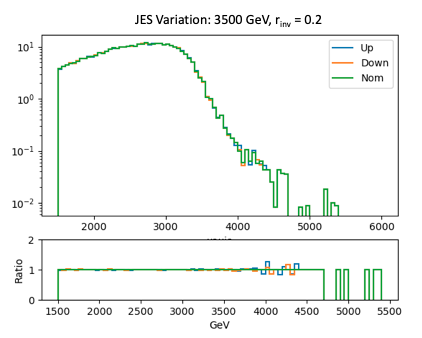
\includegraphics[width=0.6\textwidth]{figures/results/jes}
    \caption{\mt~of the 3500 GeV $Z'$, \rinv~= 0.2 signal point, shown with an example JES noise uncertainty variation. The nominal shape, 1$\sigma$ up, and 1$\sigma$ down variations are shown. The variation is seen to have minimal impact on the signal shape. Signal only (no background) is shown. 
    \label{fig:jes_uncert}}
\end{figure}

To make a conservative estimate of their impact on the shape, all shape uncertainty sources are summed in quadrature, bin-by-bin.
This results in a maximum 1$\sigma$ ``up'' variation and a maximum 1$\sigma$ ``down'' variation. 
The the impact of these maximal shape variations on the $Z'$ production cross section limit is evaluated, and uncertainty on this limit is propagated to the final limit bands. 
The impact is generally seen to be quite small, changing the limit variation by 0.61 fb at most. 
An example of the variations summed in quadrature is shown in Figure~\ref{fig:jetcp_sumq}. 
\begin{figure}[!htbp]
\centering
   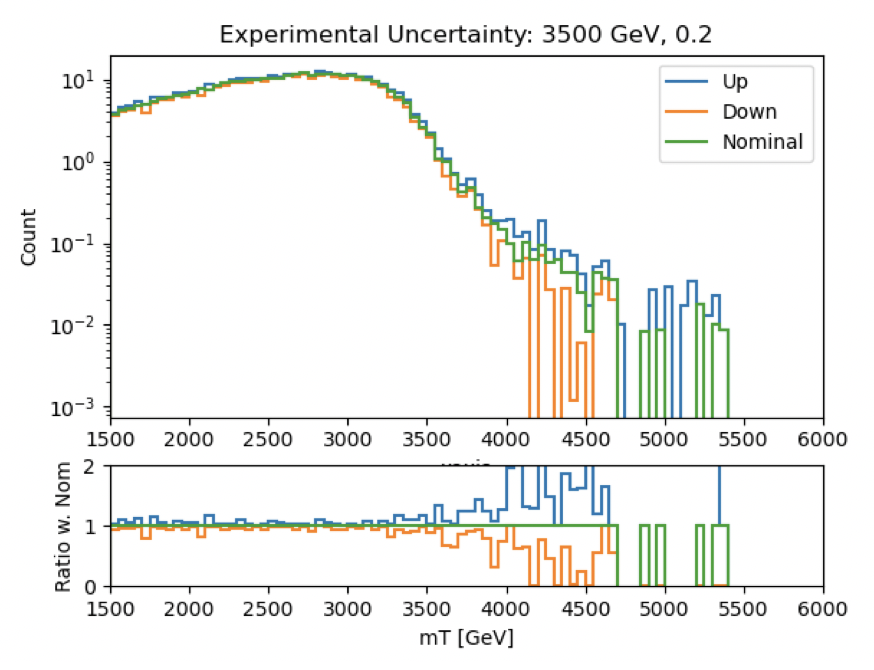
\includegraphics[width=0.62\textwidth]{figures/results/jetcp_sumq}
    \caption{\mt~of the 3500 GeV $Z'$, \rinv~= 0.2 signal point, shown with the sum in quadrature of all JES and JER variations. The nominal shape before systematic variations, the maximal 1$\sigma$ ``up", and maximal 1$\sigma$ ``down" variations are shown. Even summed in quadrature, the effect of the JES and JER variations on the shape of the signal is seen to be small.
    \label{fig:jetcp_sumq}}
\end{figure}

%------------------------------------------------------------
\subsubsection{Theory Uncertainty}
Uncertainty on the parameters of the signal model are also considered. 
The primary theory uncertainty source is the tuning of the parton shower in \textsc{Pythia8} \cite{parton_shower}. 
Jet structure and extra jet production within the event depend on the modeling of initial state radiation (ISR), final state radiation (FSR) and behavior of multiple parton interactions (MPI) within an event.
A variety of MC generation tuning parameters govern the behavior of ISR, FSR and MPI in the signal generation.
Ref~\cite{pythia8_tunes} describes how these parameters are condensed into 10 variations which capture the maximal range of impact for these tuning parameters. 

The 10 variations (representing 5 up/down variation pairs) are evaluated for the SVJ signal shapes. 
Figure~\ref{fig:isrfsr} provides a look at the effect of these variations on the SVJ \mt~signal shape. 

\begin{figure}[!htbp]
\centering
   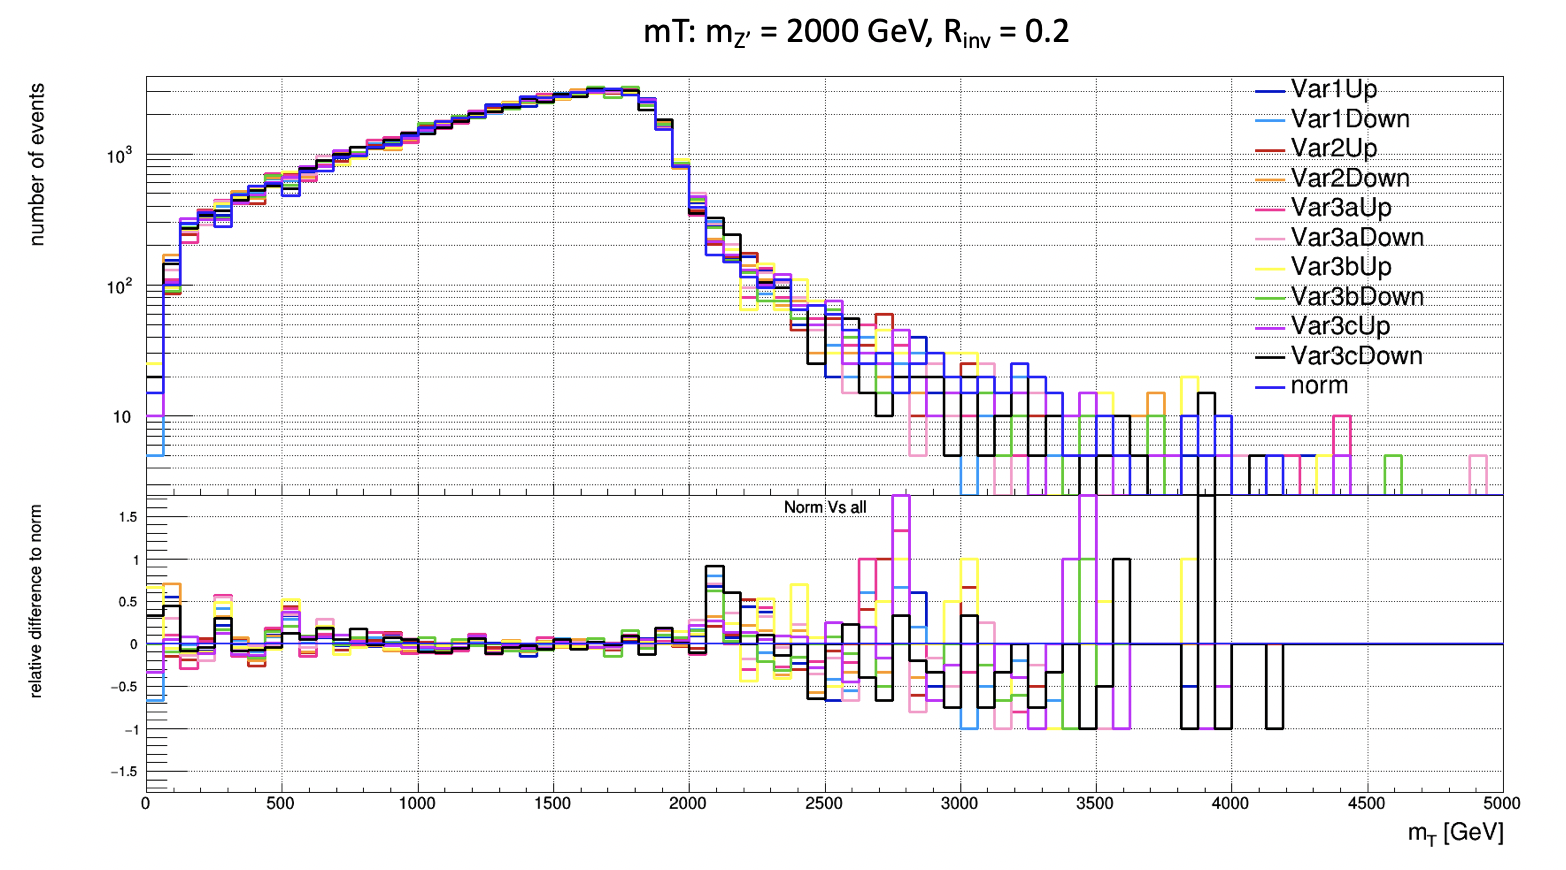
\includegraphics[width=0.9\textwidth]{figures/systs/isrfsr}
    \caption{Signal distribution of \mt, varying the ISR (Var1), FSR (Var2) and MPI (Var3a-c) configurations.
    \label{fig:isrfsr}}
\end{figure}

There is no substantial sculpting of the \mt~shape from any of the 10 systematic variations.
Particularly through the core of the distribution, the net impact of the variations is flat.
thus the systematic is considered for its impact on the signal yield.
The variation in the signal yield is at most 1.2\%.
A conservative 2\% yield uncertainty is applied to account for the uncertainty on the theory model.
The spurious signal uncertainty is dominant for all but the lowest mass signal points.

%------------------------------------------------------------
\subsection{Interpretation}
Using a modified frequentist approach \cite{freq}, \textit{exclusion limits} at the 95\% confident level (CL) are derived.
The process was first described in Section~\ref{subsec:fit_expsens} and is reviewed here.
Exclusion limits refer to determining the maximum (or \textit{limiting}) signal cross section compatible with the observed data spectrum, such that any theory resulting in a signal cross section above the limit is excluded with 95\% confidence. 
The limit is determined from a maximum likelihood test statistic \cite{likelihood}, which determines the likelihood of observing the given data spectrum using the background hypothesis, signal hypothesis, and uncertainty parameters.
Compatibility of the signal model with the observed distribution is tested by generating pseudo-data based on the background estimation and including varying amounts of signal.
Through analysis of these pseudo-data experiments, the maximum number of signals events that is compatible with the observed data distribution and background estimation can be determined.
The 95\% confidence level is enforced by dictating that the number of signal events must be compatible with the observed data within 2$\sigma$ of uncertainty.

The final limits on the $Z'$ cross section after the implementation of the systematic uncertainties are shown in Figure~\ref{fig:unblinded_limits_syst}. 
\begin{figure}[!htbp]
\centering
   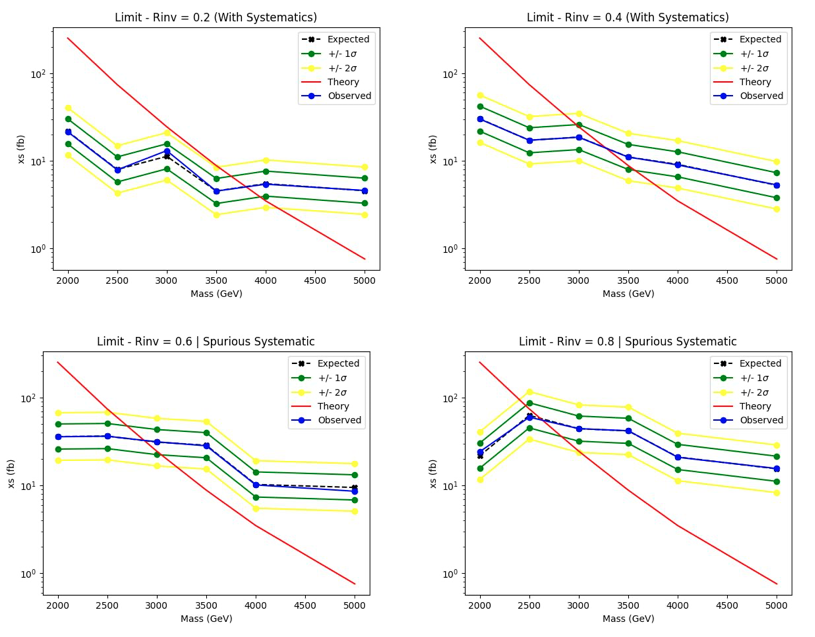
\includegraphics[width=0.95\textwidth]{figures/results/final_limits}
    \caption{Expected and observed 95\% C.L. limits in the unblinded SR, as a function of $Z'$ mass for \rinv~= 0.2 (top left), 0.4 (top right), 0.6 (bottom left), 0.8 (bottom right). The red line indicates the theoretical cross section, while the blue line indicates the observed 95\% C.L. upper limit on the cross section given the data spectrum. The black line indicates the expected limit given the background shape provided by the fit. The green and yellow bands indicate the uncertainty bands.
    \label{fig:unblinded_limits_syst}}
\end{figure}
Exclusion of the theoretical model is observed for the 2000 GeV $Z'$ mass point for all \rinv~ values.
We are unable to exclude the highest mass points due to their low theoretical cross section, and relatively high spurious signal uncertainty.
The most mass points are excluded for \rinv~= 0.2, which excludes $Z'$ masses up to 3500 GeV.

\clearpage
%--------------------------------------------------------
\section{Discovery Result}
\label{sec:results_svj}
Figure~\ref{fig:unblinded_antelope_masked} shows the unblinded \mt~spectrum in the Discovery SR with a background-only fit, and the resulting BumpHunter test.
The polynomial fit is successful and has a background-only p-value of 0.74, indicating the data is compatible with the background hypothesis. 
The BumpHunter test gives a p-value of 0.8098, indicating no significant excess.
The maximum local significance is 0.877$\sigma$, located at 1700 GeV.

\begin{figure}[!htbp]
\centering
   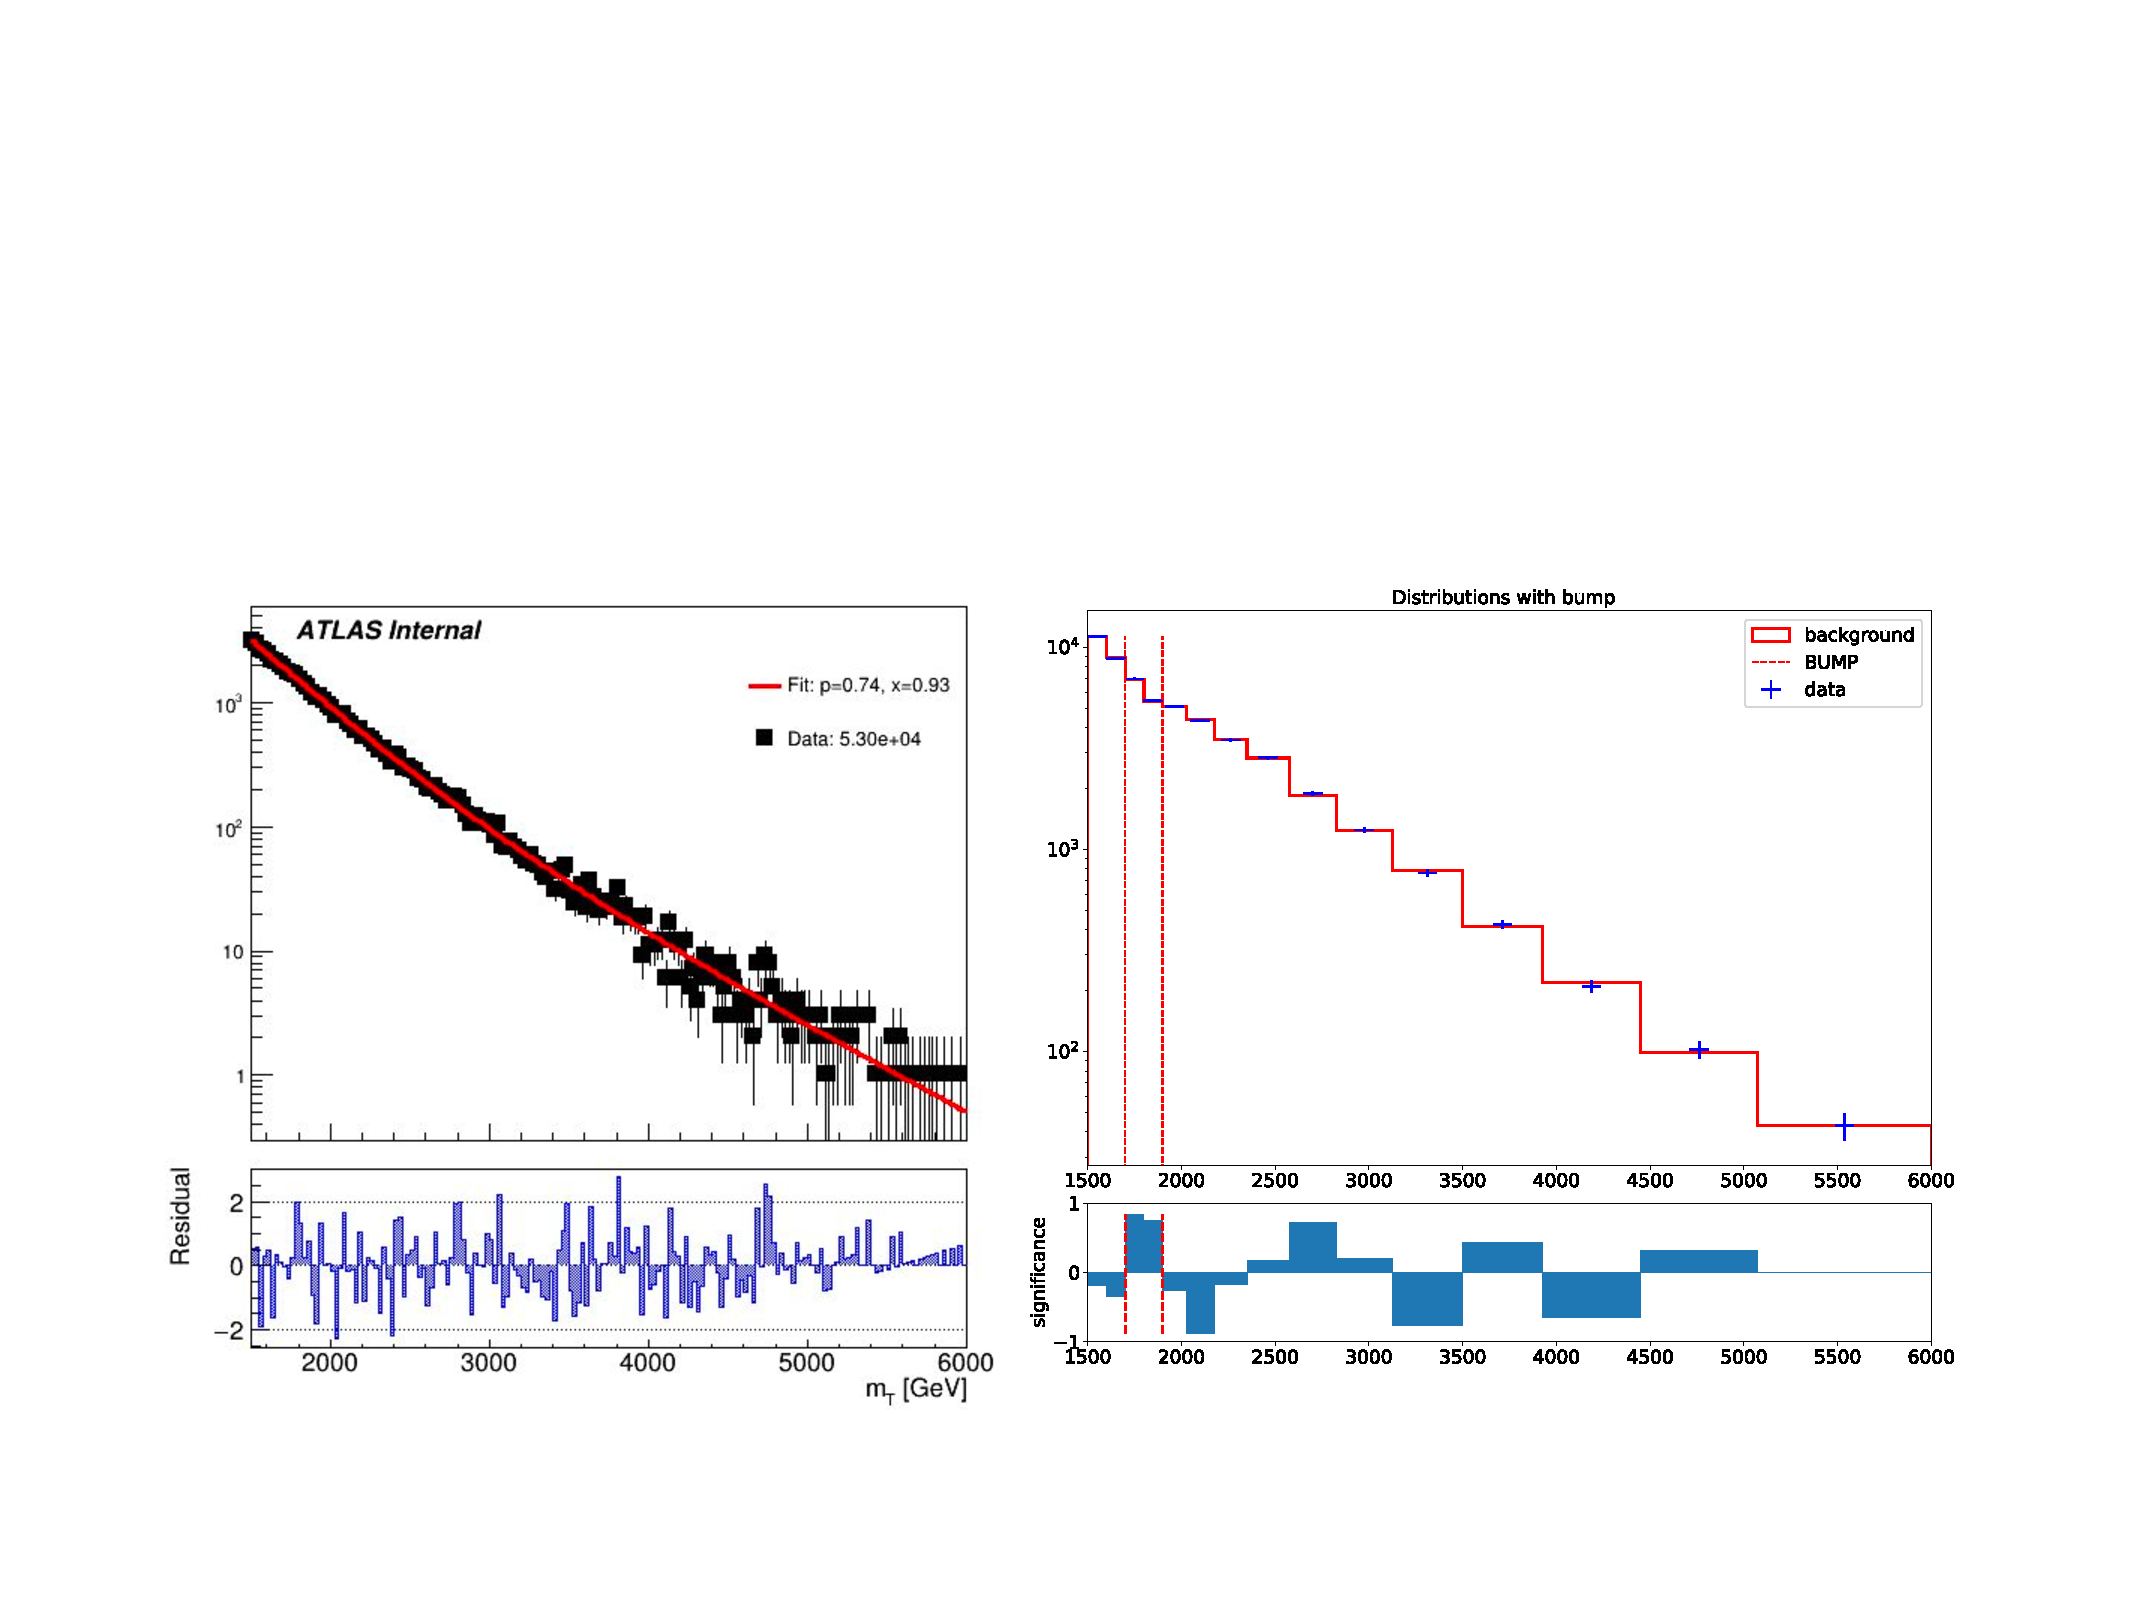
\includegraphics[width=0.95\textwidth]{figures/results/unblinded_antelope_unmasked}
    \caption{\mt~in the unblinded ANTELOPE SR with a background-only fit (p-value = 0.74), left. BumpHunter test selecting the most significant data excess with a p-value of 0.8098, right.
    \label{fig:unblinded_antelope_masked}}
\end{figure}

Because there is no specific signal interpretation for the Discovery region and both the polynomial fit and BH analysis are entirely data driven, there are no systematics to consider in the interpretation of the BH result.
%To further characterize the ANTELOPE \mt~spectrum, the bin interval of most significant deviation as identified by the BumpHunter test is masked, and the fit is rerun.
%The resulting polynomial fit has an improved p-value of 0.86, as anticipated, indicating good fit response (Figure~\ref{fig:unblinded_antelope_masked}.
%\begin{figure}[!htbp]
%\centering
%   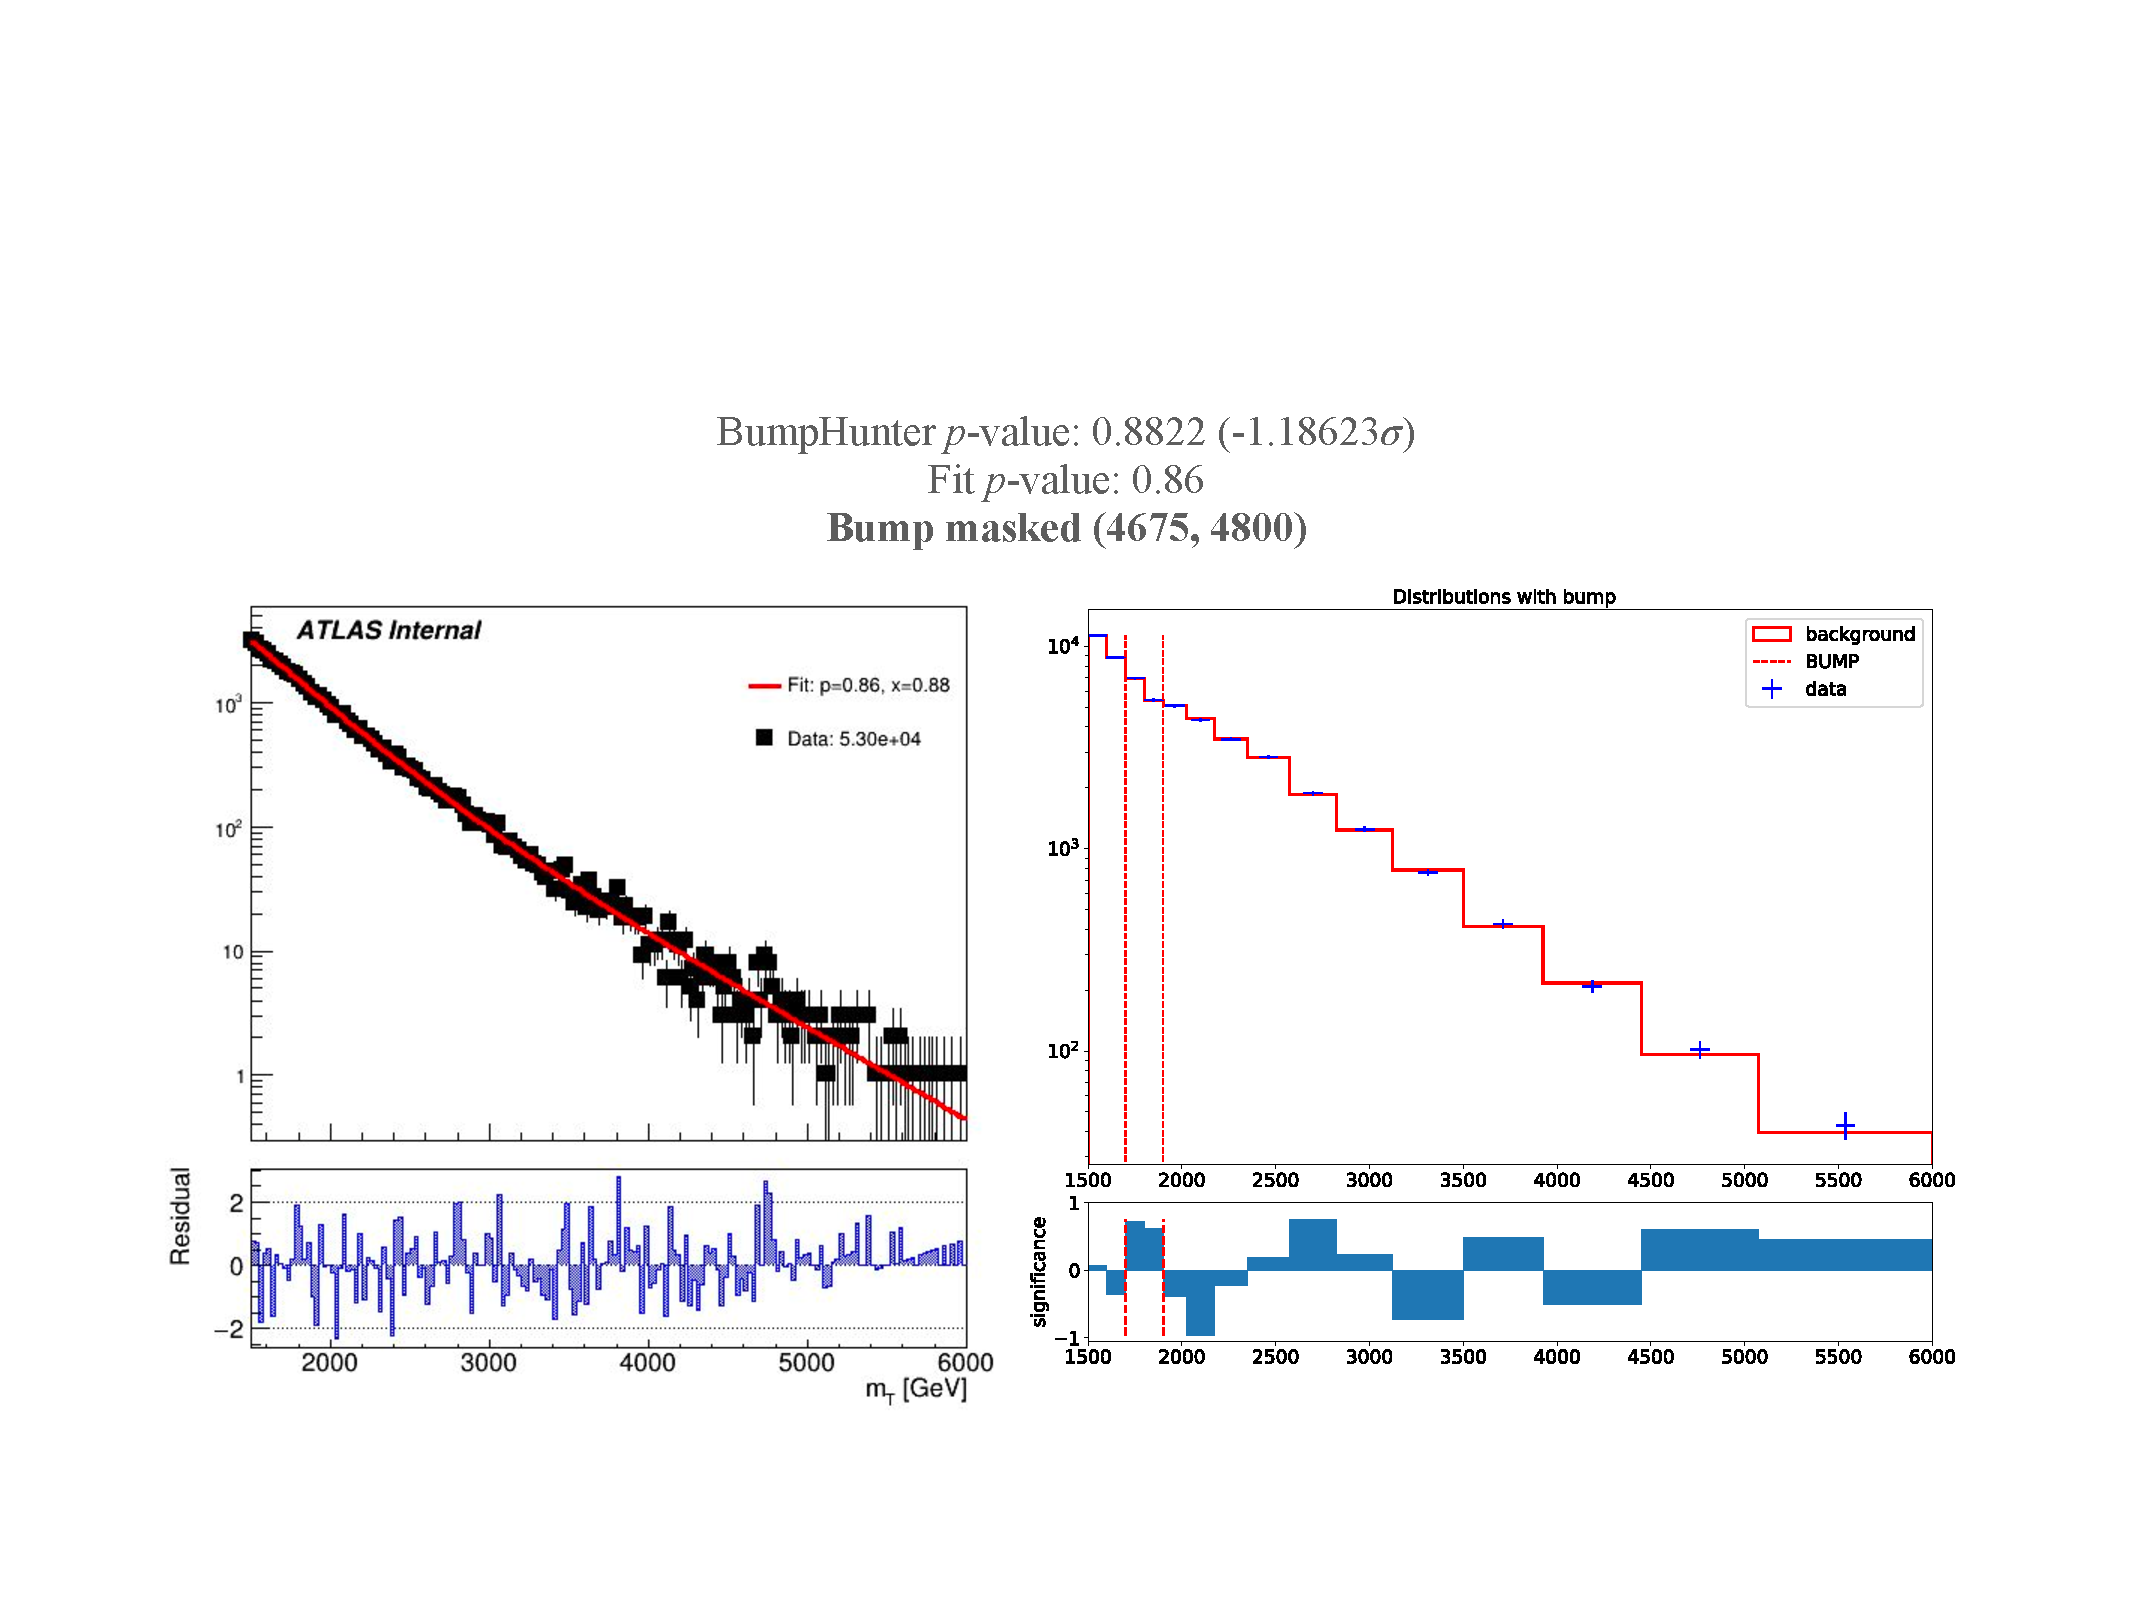
\includegraphics[width=0.5\textwidth]{figures/results/unblinded_antelope_masked}
%    \caption{\mt~in the unblinded and BH masked ANTELOPE SR with a new background-only fit (p-value = 0.86, indicating improved compatibility), left. BumpHunter test selecting the most significant data excess with a p-value of 0.8822 (eg. less significant than unmasked).
%    \label{fig:unblinded_antelope_unmasked}}
%\end{figure}

